\documentclass{article}
\usepackage{graphicx}
\usepackage{array}
\usepackage{geometry}
\geometry{a4paper, margin=1in}

\begin{document}

\begin{figure}
    \centering
    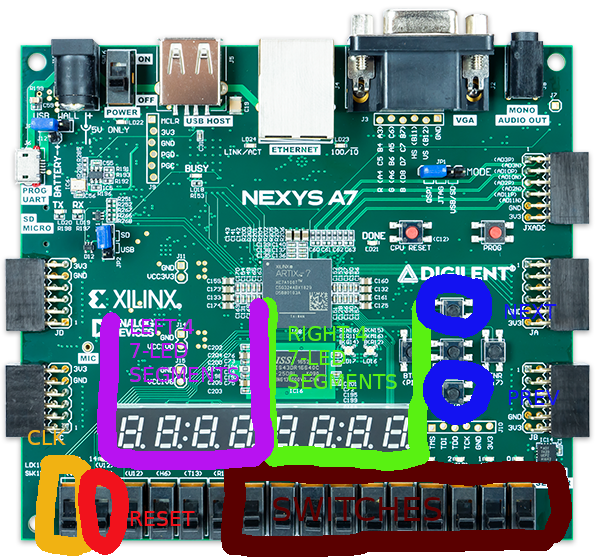
\includegraphics[width=0.8\textwidth]{nexys-a7-top_mod.png}
    \caption{FPGA Board Top View}
    \label{fig:fpga}
\end{figure}

\begin{table}[h!]
    \centering
    \begin{tabular}{|c|c|c|c|}
        \hline
        \textbf{State} & \textbf{Switches} & \textbf{Left 4 7-LED Segments} & \textbf{Right 4 7-LED Segments} \\
        \hline
        REGS & [3:0] REG Address& Register Name (Table \ref{tab:registers}) & Register Value\\
        \hline
        RAM & [9:0] RAM Address& rAM & Ram Value\\
        \hline
        BUS & NA & bUS & Bus Value\\
        \hline
        FSM & NA & FSM & FSM State (Table \ref{tab:fsm_states})\\
        \hline
    \end{tabular}
    \caption{State Display Table}
    \label{tab:state_display}
\end{table}


\begin{table}[h!]
    \centering
    \begin{tabular}{|c|c|c|}
        \hline
        \textbf{Register Name} & \textbf{Address Value} & \textbf{7-Segment Display Name} \\
        \hline
        RA & 0x0 & rrA \\
        \hline
        RB & 0x1 & rrB \\
        \hline
        RC & 0x2 & rrC \\
        \hline
        SP & 0x3 & rSP \\
        \hline
        XA & 0x4 & rXA \\
        \hline
        XB & 0x5 & rXb \\
        \hline
        BA & 0x6 & rbA \\
        \hline
        BB & 0x7 & rbb \\
        \hline
        PC & 0x8 & rPC \\
        \hline
        FR & 0x9 & rFr \\
        \hline
        MA & 0xA & rMA \\
        \hline
        IOA & 0xB & rIO \\
        \hline
        T1 & 0xC & rT1 \\
        \hline
        T2 & 0xD & rT2 \\
        \hline
        IR & 0xE & rIr \\
        \hline
        Nothing & 0xF &  \\
        \hline
    \end{tabular}
    \caption{Register Address and 7-Segment Display Names}
    \label{tab:registers}
\end{table}

\begin{table}[h!]
    \centering
    \begin{tabular}{|l|c|c|}
        \hline
        \textbf{FSM State} & \textbf{Hex Value} & \textbf{FSM 7-LED Segment Name} \\
        \hline
        RESET & 0x00 & rSt \\
        \hline
        FETCH & 0x10 & FEt \\
        \hline
        FETCH1 & 0x11 & FEt1 \\
        \hline
        FETCH2 & 0x12 & FEt2 \\
        \hline
        DECODE & 0x20 & dCd \\
        \hline
        ADDR\_SUM & 0x30 & AdS \\
        \hline
        ADDR\_SUM1 & 0x31 & AdS1 \\
        \hline
        ADDR\_SUM2 & 0x32 & AdS2 \\
        \hline
        ADDR\_REG & 0x34 & Adr \\
        \hline
        ADDR\_IO & 0x3c & AdI \\
        \hline
        LOAD\_SRC\_REG & 0x40 & LSr \\
        \hline
        LOAD\_SRC\_MEM & 0x44 & LSm \\
        \hline
        LOAD\_SRC\_MEM1 & 0x45 & LSm1 \\
        \hline
        LOAD\_SRC\_MEM2 & 0x46 & LSm2 \\
        \hline
        LOAD\_SRC\_IO & 0x4c & LSI \\
        \hline
        LOAD\_SRC\_IO1 & 0x4d & LSI1 \\
        \hline
        LOAD\_DST\_REG & 0x50 & Ldr \\
        \hline
        LOAD\_DST\_MEM & 0x54 & Ldm \\
        \hline
        LOAD\_DST\_MEM1 & 0x55 & Ldm1 \\
        \hline
        LOAD\_DST\_MEM2 & 0x56 & Ldm2 \\
        \hline
        NO\_LOAD\_DST\_REG & 0x60 & ndr \\
        \hline
        NO\_LOAD\_DST\_IO & 0x6c & ndi \\
        \hline
        EXEC\_ONE\_OP & 0x70 & E10 \\
        \hline
        EXEC\_TWO\_OP & 0x74 & E20 \\
        \hline
        EXEC\_TRANSFER & 0x78 & ET \\
        \hline
        STORE\_REG & 0x80 & Str \\
        \hline
        STORE\_MEM & 0x84 & Stm \\
        \hline
        STORE\_MEM1 & 0x85 & Stm1 \\
        \hline
        STORE\_IO & 0x8c & StI \\
        \hline
        INC\_PC & 0x90 & IPC \\
        \hline
        INC\_PC1 & 0x91 & IPC1 \\
        \hline
    \end{tabular}
    \caption{FSM States and Corresponding Hex Values and 7-LED Segment Names}
    \label{tab:fsm_states}
\end{table}




\end{document}